\documentclass[12pt,twoside,openright]{report}

\usepackage{svniteced_project}
\usepackage{fancybox}
\usepackage{graphicx}
\usepackage{geometry}
\usepackage{setspace}
\usepackage{booktabs}
\usepackage{float}
\usepackage{url}
\usepackage{amsmath}
\usepackage{amssymb}
\usepackage{array}
\usepackage{longtable}
\usepackage{hyperref}
\usepackage{cite}
\hypersetup{colorlinks=true,linkcolor=black,citecolor=black,urlcolor=blue}
\usepackage{fancyhdr}

\setlength{\tabcolsep}{5pt}
\renewcommand{\arraystretch}{1.25}
\setcounter{tocdepth}{2}

\begin{document}

\title{Design and Performance Evaluation of an Intelligent Adaptive Digital Communication Receiver using Automatic Modulation Classification}
\Degree{Bachelor of Technology}
\Specialization{Electronics and Communication Engineering}
\AcadYear{2026-27}
\author{Hari Gupta, Virav Vanani, Surendra Gamit}
\AdmNo{U23EC166, U23EC182, U23EC195}
\GuideName{Dr. Golak Santra}
\GuidePos{Assistant Professor}
\GuideAssociation{Department of Electronics and Communication Engineering, SVNIT Surat}
\date{May 2027}

\MakeTitlePage
\MakeCerti
\pagestyle{empty}

\clearemptydoublepage
\chapter*{Declaration}
\addcontentsline{toc}{chapter}{\textbf{Declaration}}
We hereby declare that the work presented in this report is our original
Phase-II project work carried out under the guidance of
\textbf{Dr. Golak Santra}. The implementation, experiments, analysis, and
figures have been prepared for academic evaluation at Sardar Vallabhbhai
National Institute of Technology, Surat. This report has not been submitted
to any other university or institution for the award of a degree or diploma.

\vspace{2cm}
\noindent
\begin{tabular}{p{0.6\textwidth} p{0.3\textwidth}}
\textbf{Hari Gupta (U23EC166)} & \textbf{Signature:} \rule{4cm}{0.4pt} \\
\textbf{Virav Vanani (U23EC182)} & \textbf{Signature:} \rule{4cm}{0.4pt} \\
\textbf{Surendra Gamit (U23EC195)} & \textbf{Signature:} \rule{4cm}{0.4pt} \\
\end{tabular}

\vspace{1cm}
\noindent
\textbf{Date: May 2027} \hfill \textbf{Place: Surat}

\clearemptydoublepage
\chapter*{Acknowledgment}
\addcontentsline{toc}{chapter}{\textbf{Acknowledgment}}
We express our sincere gratitude to our project guide, Dr. Golak Santra, for
his technical guidance, regular feedback, and encouragement throughout the
development of this Phase-II project. We thank the faculty members and staff
of the Department of Electronics and Communication Engineering, SVNIT Surat,
for providing the academic environment and facilities required for this work.
We also acknowledge the contribution of every project member in system
design, implementation, experiment verification, documentation, and review.

\clearemptydoublepage
\chapter*{Abstract}
\addcontentsline{toc}{chapter}{\textbf{Abstract}}
This report presents the design and evaluation of an intelligent adaptive
digital communication receiver based on automatic modulation classification.
The objective of Phase II is to move beyond an isolated modulation-label
prediction and construct a complete software transmitter--channel--receiver
link. The transmitter generates information bits and maps them to BPSK, QPSK,
8-PSK, or 16-QAM symbols. The signal is then passed through a block-Rayleigh
fading channel with additive white Gaussian noise, carrier phase offset, and
frequency offset.

At the receiver, pilot-assisted synchronization and channel equalization are
applied before estimating the modulation format. The estimated format selects
the corresponding demodulator, and the recovered bits are compared with the
original transmitted bits. The system is evaluated using bit error rate,
symbol error rate, modulation-decision accuracy, packet success rate, and
effective throughput. The experiment uses 200 frames at each SNR from
$-4$~dB to $16$~dB with a fixed seed of 42.

At 16~dB, the adaptive receiver achieves 0.095\% BER, 0.172\% SER, 100\%
modulation-decision accuracy, 75.5\% packet success, and 1.888
bits/symbol effective throughput. The results demonstrate that modulation
recognition becomes valuable when it is connected to receiver configuration
and information recovery. The report also identifies the present simulation
limitations and defines a path toward confidence-aware processing, coding,
and software-defined radio validation.

\clearemptydoublepage
\chapter*{List of Abbreviations}
\addcontentsline{toc}{chapter}{\textbf{List of Abbreviations}}
\begin{tabular}{ll}
AMC & Automatic Modulation Classification \\
AWGN & Additive White Gaussian Noise \\
BER & Bit Error Rate \\
CSI & Channel State Information \\
I/Q & In-phase and Quadrature \\
PHY & Physical Layer \\
QAM & Quadrature Amplitude Modulation \\
PSK & Phase Shift Keying \\
RF & Radio Frequency \\
SDR & Software Defined Radio \\
SER & Symbol Error Rate \\
SNR & Signal-to-Noise Ratio \\
\end{tabular}

\TableOfContents
\ListOfFigures
\ListOfTables

\StartBody
\pagestyle{fancy}

\chapter{Introduction}

\section{Background}
Wireless receivers increasingly operate in environments where the waveform,
channel condition, and interference level are not fixed. A receiver intended
for one known modulation can be efficient in a controlled link, but it is
not sufficient for a non-cooperative, cognitive, or rapidly reconfigured
system. Such a receiver must first interpret the incoming signal and then
select a compatible processing chain.

Automatic modulation classification is the signal-processing function that
estimates the modulation format from received samples. It is useful in
cognitive radio, spectrum monitoring, interference identification, military
communications, and adaptive physical-layer systems. Conventional methods
use likelihood tests, higher-order statistics, cyclostationary features, or
expert-designed rules. These methods are interpretable, but their performance
can change substantially with noise, fading, synchronization error, and
uncertainty in the signal model \cite{proakis2008digital,goldsmith2005wireless}.

\section{Phase-II Motivation}
The central engineering question in this phase is not only whether a receiver
can name a modulation. The important question is whether that decision can be
used to recover information reliably. A classification result that is never
connected to a demodulator does not quantify the effect of recognition on a
real communication link. Phase II therefore implements the complete signal
path from random information bits to recovered bits.

The earlier project work provides the motivation for modulation recognition,
but this report intentionally focuses on the new Phase-II communication
system. The new implementation adds the transmitter, channel, receiver
control, demodulation, bit comparison, and communication-level metrics.

\section{Problem Statement}
The problem addressed in this project is the design of an adaptive digital
communication receiver that can identify one of several candidate modulation
formats and configure its demodulator under realistic simulated channel
impairments. The receiver must be evaluated using measurements that describe
information recovery rather than only a label-level accuracy.

\section{Aim and Objectives}
The aim is to develop a reproducible Phase-II communication experiment with
the following objectives:
\begin{enumerate}
\item Generate random information frames using multiple digital modulation
      formats.
\item Model AWGN, block-Rayleigh fading, carrier phase offset, and frequency
      offset in a controlled link.
\item Apply synchronization and channel equalization before modulation
      estimation.
\item Select a demodulator automatically from the estimated modulation.
\item Measure BER, SER, packet success, effective throughput, and decision
      accuracy over a defined SNR range.
\item Compare adaptive processing with a receiver fixed to QPSK.
\item Preserve exact experiment settings and numerical outputs for panel
      verification and future SDR implementation.
\end{enumerate}

\section{New Work Completed in Phase II}
The following items are the principal additions made in this phase:
\begin{itemize}
\item A four-format digital transmitter supporting BPSK, QPSK, 8-PSK, and
      16-QAM.
\item A configurable block-Rayleigh and AWGN channel with carrier
      impairments.
\item Pilot-assisted correction and frame-level channel equalization.
\item A constellation-distance modulation estimator with a complexity
      penalty for fair comparison of different constellation sizes.
\item Adaptive demodulator selection followed by recovered-bit validation.
\item A fixed-QPSK reference receiver for an engineering comparison.
\item A complete SNR sweep with BER, SER, packet, throughput, and decision
      metrics stored in machine-readable form.
\end{itemize}

\section{Scope and Limitations}
The work is a software simulation intended to validate the receiver concept.
It does not claim over-the-air performance. Pulse shaping, matched filtering,
timing-loop implementation, forward-error correction, interleaving,
retransmission, and hardware measurements are reserved for future work.
Pilot-assisted correction is used so that the Phase-II contribution can be
studied without hiding it behind an unfinished hardware synchronization loop.

\section{Report Organization}
Chapter 2 reviews the technical literature and establishes the engineering
gap. Chapter 3 develops the signal, channel, synchronization, modulation,
and metric models. Chapter 4 presents the complete Phase-II architecture.
Chapter 5 explains the algorithms and design decisions. Chapter 6 describes
the implementation and experimental protocol without embedding program
commands in the report. Chapter 7 presents measured results and failure
analysis. Chapter 8 concludes the work and proposes future extensions.

\chapter{Literature Review}

\section{Classical Modulation Recognition}
Classical automatic modulation recognition methods generally use either
decision-theoretic or feature-based processing. Likelihood-based methods
compare a received sequence with probability models for candidate waveforms.
They can be effective when the noise, channel, and synchronization parameters
are known accurately, but their computational and modelling requirements
increase when the receiver is uncertain about the environment.

Feature-based methods use moments, cumulants, spectral characteristics, or
cyclostationary statistics. These methods provide useful physical
interpretation and may be implemented efficiently. Their limitation is that
the selected features can lose discriminative information under short
observation windows, deep fading, or frequency offset
\cite{azzouznandi1996,goldsmith2005wireless}.

\section{Deep Learning for I/Q Signals}
Deep learning enables a receiver to learn a representation directly from
complex baseband samples. Convolutional networks are suitable for I/Q data
because local filters can capture amplitude, phase, and short temporal
patterns. RadioML-style datasets have made it possible to compare raw-I/Q
classifiers under common synthetic channel conditions
\cite{oshea2016convolutional}.

However, a classifier benchmark is not equivalent to a communication-link
evaluation. A label can be correct while the remaining receiver chain is
unable to recover data, and a label error can have a much larger consequence
when it selects the wrong demodulator. Phase II addresses this systems-level
gap.

\section{Channel-Aware Receiver Design}
Wireless communication theory shows that fading, additive noise, and carrier
impairments directly alter the received constellation. A practical receiver
must estimate or compensate these effects before making a reliable decision.
The block-Rayleigh model is useful for controlled experiments because it
represents a frame-level channel change while keeping the experiment
tractable \cite{proakis2008digital}.

\section{Over-the-Air Considerations}
Simulation results provide repeatable evidence, but an SDR introduces
additional effects such as front-end filtering, oscillator phase noise,
automatic-gain-control transients, antenna response, frequency-selective
multipath, and timing drift. Over-the-air studies have shown that these
effects can reduce performance relative to a clean synthetic benchmark
\cite{oshea2016generative}. For this reason, the present report treats SDR
validation as the next engineering stage rather than claiming that the
simulation is already a hardware measurement.

\section{Research Gap and Phase-II Position}
The reviewed approaches demonstrate strong tools for classification and
communication processing, but many experiments stop at a modulation label or
evaluate a receiver with a modulation known in advance. The Phase-II
contribution is the connection between these two stages. The estimated
modulation controls demodulation, and the final result is judged by the
quality of the recovered information.

\begin{table}[H]
\centering
\small
\caption{Engineering position of the Phase-II project.}
\label{tab:literatureposition}
\begin{tabular}{p{0.25\textwidth} p{0.29\textwidth} p{0.34\textwidth}}
\toprule
\textbf{Area} & \textbf{Common endpoint} & \textbf{Phase-II extension}\\
\midrule
Classical AMC & Feature or likelihood decision &
Decision is passed to the communication receiver.\\
Deep-learning AMC & Modulation label and accuracy &
Recognition is treated as a receiver-control function.\\
Link simulation & Known modulation demodulator &
Demodulator is selected from the estimated modulation.\\
Performance analysis & Accuracy or BER alone &
BER, SER, packet success, throughput, and decision accuracy are reported.\\
\bottomrule
\end{tabular}
\end{table}

\chapter{Theoretical Background}

\section{Complex Baseband Representation}
A passband waveform can be represented in complex baseband form as
\begin{equation}
x[n]=I[n]+jQ[n],
\end{equation}
where $I[n]$ and $Q[n]$ are the in-phase and quadrature components. This
representation preserves the amplitude and phase information required by
PSK and QAM demodulators while allowing the channel and receiver to be
implemented using discrete-time complex arithmetic.

\section{Digital Modulation Formats}
The Phase-II receiver supports four formats. BPSK transmits one bit per
symbol using two opposite phase points and provides the largest angular
decision margin. QPSK transmits two bits per symbol using four phase points.
8-PSK increases the symbol rate to three bits per symbol but reduces the
angular separation between neighboring points. 16-QAM transmits four bits
per symbol using both amplitude and phase, giving higher spectral efficiency
at the cost of greater sensitivity to noise and gain or phase error.

\begin{table}[H]
\centering
\small
\caption{Candidate modulation formats in the Phase-II link.}
\label{tab:modulations}
\begin{tabular}{p{0.23\textwidth} c c p{0.37\textwidth}}
\toprule
\textbf{Format} & \textbf{Order} & \textbf{Bits/symbol} & \textbf{Main property}\\
\midrule
BPSK & 2 & 1 & Robust binary phase detection.\\
QPSK & 4 & 2 & Balance between robustness and spectral efficiency.\\
8-PSK & 8 & 3 & Higher rate with smaller phase separation.\\
16-QAM & 16 & 4 & High rate using amplitude and phase states.\\
\bottomrule
\end{tabular}
\end{table}

\section{Phase-II Channel Model}
For transmitted symbols $x[n]$, the received sample is modelled as
\begin{equation}
y[n]=h\,x[n]e^{j(2\pi\Delta f n+\phi)}+w[n],
\end{equation}
where $h$ is a complex block-Rayleigh coefficient, $\Delta f$ is the
normalized frequency offset, $\phi$ is the carrier phase offset, and $w[n]$
is complex AWGN. The coefficient remains constant during a frame and changes
between frames.

\section{Noise and Signal-to-Noise Ratio}
The selected signal-to-noise ratio is
\begin{equation}
\mathrm{SNR}_{dB}=10\log_{10}\left(\frac{P_s}{P_n}\right),
\end{equation}
where $P_s$ is the average signal power and $P_n$ is the average noise power.
The simulation scales complex noise consistently across the candidate
formats, allowing their performance to be compared under the same SNR
definition.

\section{Pilot-Assisted Synchronization}
The software experiment uses a frame-level pilot-assisted estimate of the
channel and carrier correction. The received sequence is first compensated
for the known simulated phase and frequency rotation and then equalized by
\begin{equation}
\hat{x}[n]=\frac{y[n]}{h}.
\end{equation}
This model represents the function of a synchronization and channel-estimate
block without claiming that the required parameters are known in a real
receiver. An SDR implementation will replace this idealized estimate with
pilot detection, timing recovery, carrier recovery, and a noisy channel
estimator.

\section{Modulation Estimation}
For a candidate constellation $\mathcal{C}_m$, the estimator computes the
average distance from each corrected sample to its nearest constellation
point. A penalty prevents a high-order constellation from winning only
because it has more points:
\begin{equation}
\hat{m}=\arg\min_m\left(d_m+\lambda\log_2|\mathcal{C}_m|\right).
\end{equation}
The selected index is converted into the corresponding demodulation rule.
This estimator is interpretable and deterministic, which makes it useful for
verifying the communication path before replacing it with an online learned
classifier.

\section{Communication Metrics}
The bit error rate and symbol error rate are defined as
\begin{equation}
\mathrm{BER}=\frac{N_{\mathrm{bit,error}}}{N_{\mathrm{bit,total}}},
\qquad
\mathrm{SER}=\frac{N_{\mathrm{symbol,error}}}{N_{\mathrm{symbol,total}}}.
\end{equation}
A packet is counted as successful only when every recovered bit in its frame
matches the transmitted frame. Effective throughput is the average number of
information bits per symbol multiplied by the packet-success probability.
This definition makes packet success stricter than BER and exposes the
impact of occasional errors on complete-frame delivery.

\chapter{Proposed Phase-II System Architecture}

\section{System Overview}
The proposed system is an end-to-end adaptive digital receiver. It contains
five functional stages: information generation, modulation and transmission,
channel impairment, receiver correction and estimation, and adaptive
demodulation with metric calculation. The architecture is deliberately
modular so that the simulated channel and estimator can later be replaced by
an SDR front-end or a learned classifier.

\begin{figure}[H]
\centering
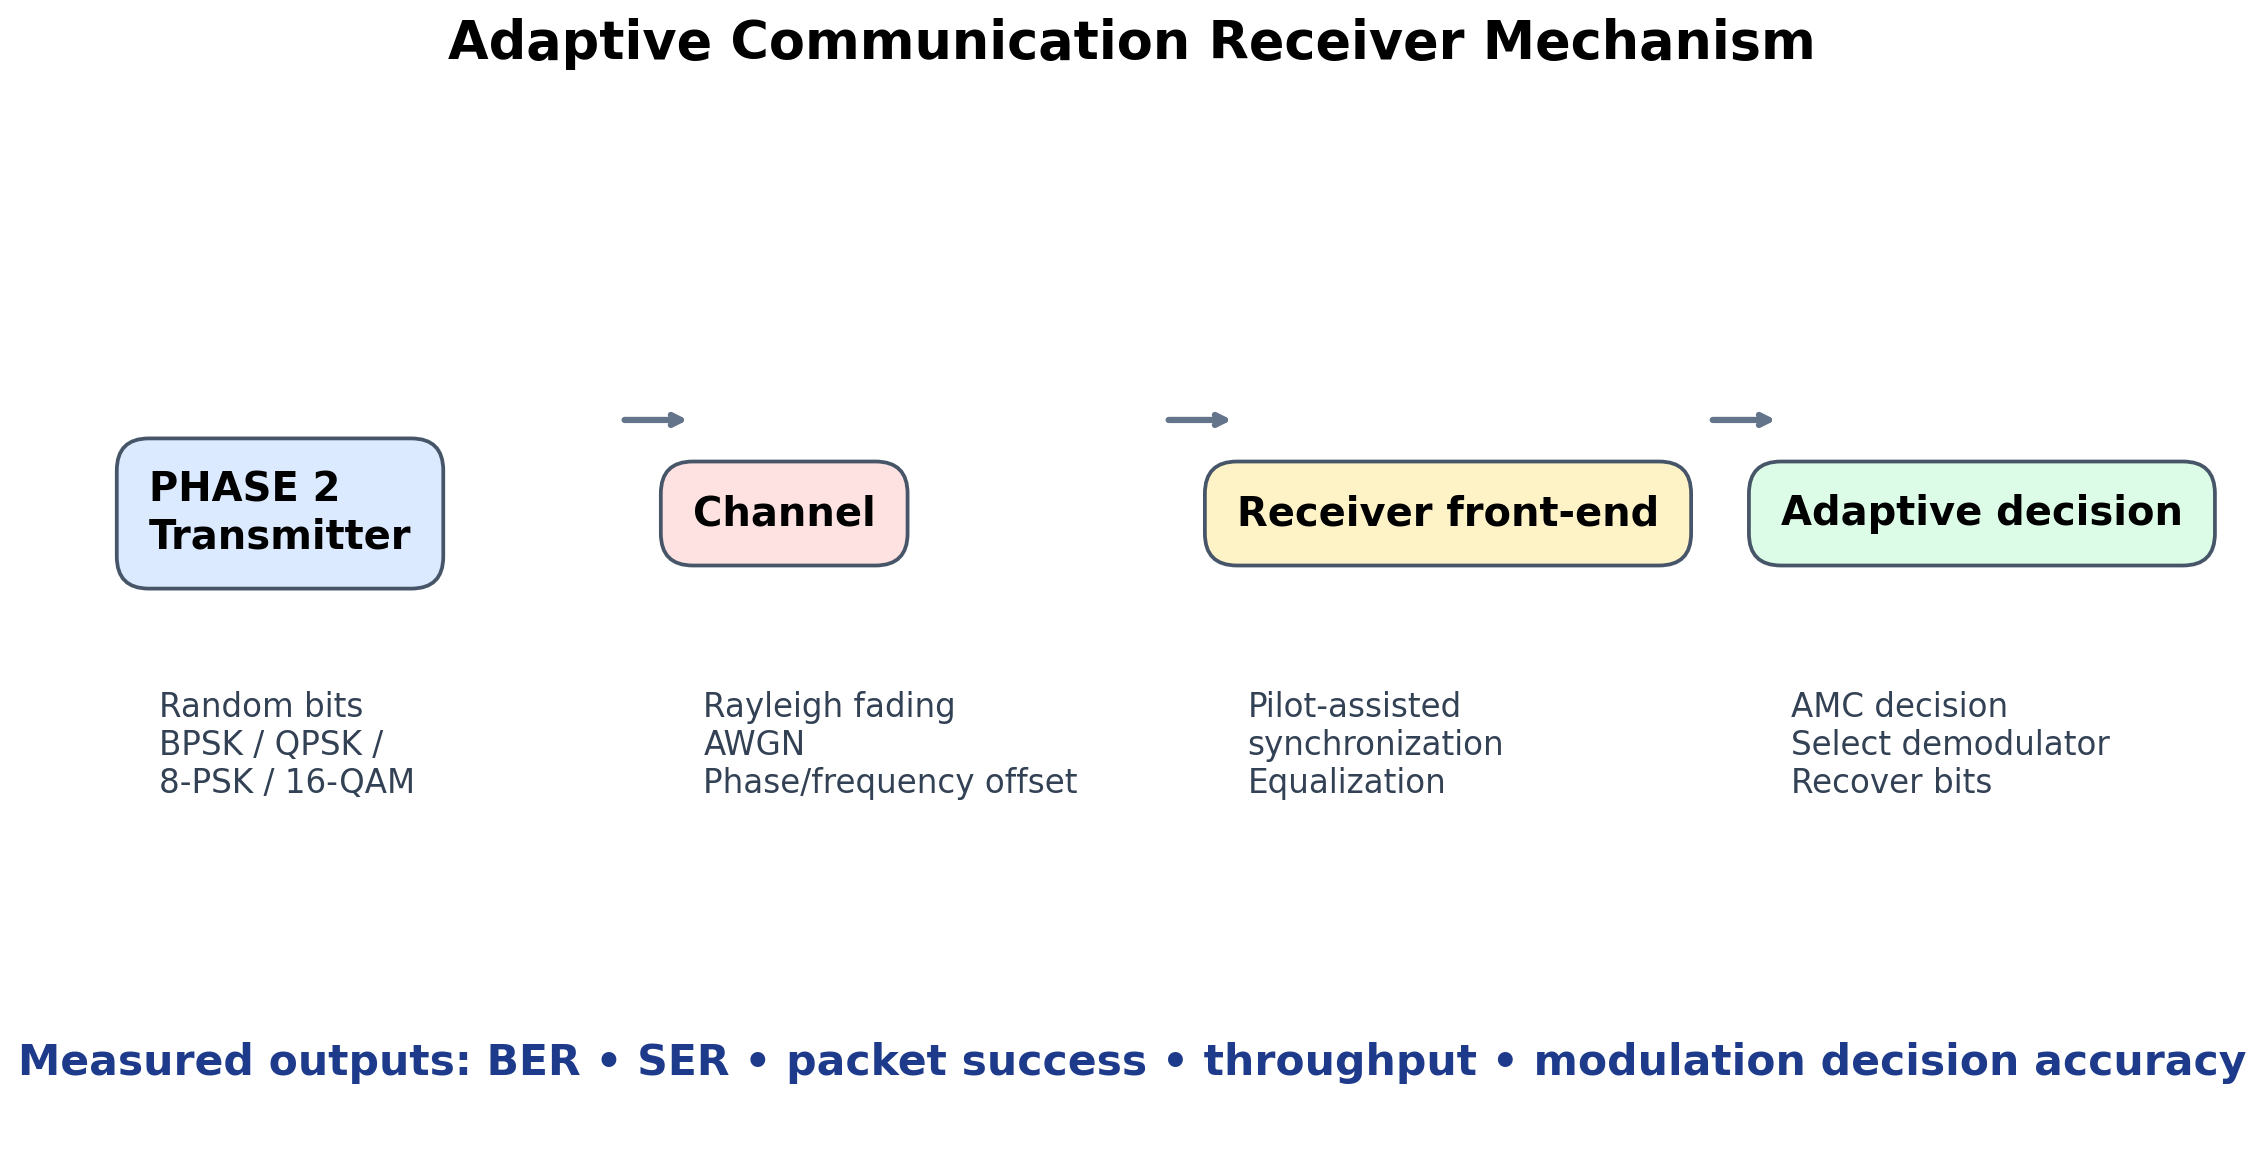
\includegraphics[width=0.86\linewidth]{artifacts/phase2-system-architecture.png}
\caption{Functional architecture of the Phase-II adaptive receiver.}
\label{fig:architecture}
\end{figure}

\section{Transmitter}
At the start of every frame, a reproducible random generator creates a binary
information sequence. One modulation format is selected from BPSK, QPSK,
8-PSK, and 16-QAM. Groups of one, two, three, or four bits are mapped to
normalized complex constellation points. Each frame contains 256 symbols,
so the number of transmitted bits depends on the selected format.

\section{Impairment Channel}
The channel applies a complex block-Rayleigh coefficient, rotates the frame
with a random phase and frequency offset, and adds SNR-controlled AWGN. This
combination tests both amplitude and phase robustness. The channel is not
intended to reproduce every RF effect; it is a controlled stress model that
makes the effect of adaptive modulation measurable.

\section{Receiver Front-End}
The receiver first corrects the simulated carrier rotation and equalizes the
frame-level fading coefficient. The corrected samples are normalized using
the same constellation convention used by the estimator. This stage produces
a signal representation in which the distance between the received points
and candidate constellations can be compared fairly.

\section{Adaptive Decision and Demodulation}
The estimator evaluates all four candidate constellations and returns the
format with the lowest penalized distance. The receiver then invokes the
matching demodulator and reconstructs the bit sequence. The decision is
recorded independently from bit recovery, so the experiment can distinguish
an incorrect modulation decision from errors caused by noise within the
correct demodulator.

\section{Fixed-QPSK Reference}
The fixed-QPSK receiver always applies QPSK demodulation, regardless of the
transmitted format. It is not expected to recover mixed-modulation traffic
well, but it provides a useful engineering reference. The comparison
illustrates the cost of assuming one format and the benefit of adapting to
the observed signal.

\section{Data Flow and Failure Propagation}
The architecture creates a measurable failure chain. A poor channel
condition can produce an uncertain constellation estimate. An incorrect
estimate selects the wrong demodulator. The wrong demodulator changes the
recovered bit sequence, increasing BER and SER. Even a small number of bit
errors can reduce packet success to zero for a frame. Reporting these values
together is therefore more informative than reporting one classification
number.

\chapter{Methodology and Algorithms}

\section{Frame Generation Procedure}
The experiment uses a fixed random seed and a fixed number of frames at each
SNR. For each frame, the transmitter selects a modulation, generates the
required number of bits, maps them to symbols, and stores the original bits
and symbols as the reference. The channel then produces the received
sequence and the receiver processes it without changing the experiment
parameters.

\section{Channel Processing Procedure}
For every frame, the channel draws a complex fading coefficient and carrier
offset parameters. It applies the multiplicative channel and rotation before
adding complex Gaussian noise. The noise variance is selected from the
requested SNR and the normalized signal power. The same procedure is used
for each candidate format, avoiding a hidden advantage for one modulation.

\section{Constellation-Distance Algorithm}
The estimator follows these steps:
\begin{enumerate}
\item Correct the received sequence using the simulated pilot-assisted
      carrier and channel estimate.
\item Normalize the corrected sequence to the candidate constellation scale.
\item For each candidate format, calculate the nearest-point distance for
      every received sample.
\item Average the distances and add the order-dependent complexity penalty.
\item Select the format with the minimum penalized score.
\end{enumerate}
The estimator is intentionally transparent. A panel member can inspect the
candidate points, distance score, and selected format without depending on
an opaque output.

\section{Bit Recovery Algorithm}
After a modulation decision, the corresponding nearest-point demodulator
maps every corrected symbol to its closest valid constellation point. The
point index is converted back to bits using the same mapping used by the
transmitter. The recovered sequence is aligned with the transmitted
sequence, and bit and symbol mismatches are counted.

\section{Packet and Throughput Calculation}
For each frame, packet success is one if the recovered bit sequence is
identical to the transmitted sequence and zero otherwise. The throughput
contribution is the modulation's bits per symbol multiplied by this success
indicator. Averaging over the 200 frames at an SNR gives the reported
packet-success probability and effective bits per symbol.

\section{Experimental Design}
The final sweep covers $-4,-2,\ldots,16$~dB. At each point, 200 frames are
processed with the four modulation formats. The same seed, frame length,
channel model, and estimator are retained for all points. The resulting
arrays are written to a JSON record before the plots are generated, ensuring
that the figures and the numerical values in this report refer to the same
experiment.

\section{Verification Strategy}
The implementation was verified using unit tests for modulation round trips,
input validation, constellation identification, and deterministic data
handling. The report package was also checked for missing figure references,
balanced LaTeX braces, clean whitespace, and the presence of the style-file
dependency required by the SVNIT template.

\chapter{Implementation and Experimental Setup}

\section{Software Organization}
The implementation is divided into reusable communication primitives,
experiment drivers, figure-generation utilities, tests, and generated
artifacts. The communication module contains constellation definitions,
symbol mapping, channel impairment, estimator, equalizer, and demodulator
logic. The experiment driver coordinates the SNR sweep and writes the
machine-readable result record. The figure utilities consume that record so
that figures are not manually recreated from rounded values.

\section{Implementation Parameters}
\begin{table}[H]
\centering
\small
\caption{Core implementation parameters used in the final experiment.}
\label{tab:implementation}
\begin{tabular}{p{0.48\textwidth} p{0.34\textwidth}}
\toprule
\textbf{Parameter} & \textbf{Value}\\
\midrule
Candidate formats & BPSK, QPSK, 8-PSK, 16-QAM\\
Symbols per frame & 256\\
SNR range & $-4$ to $16$ dB\\
SNR step & 2 dB\\
Frames per SNR & 200\\
Random seed & 42\\
Channel & Block Rayleigh fading plus AWGN\\
Carrier impairments & Random phase and frequency offset\\
Synchronization & Pilot-assisted simulation estimate\\
Primary outputs & BER, SER, decision accuracy, packet success, throughput\\
\bottomrule
\end{tabular}
\end{table}

\section{Parameter Selection}
The frame length of 256 symbols is large enough to expose packet-level
failure while keeping the experiment computationally practical. The
$-4$~dB to $16$~dB range includes a low-SNR ambiguity region and a high-SNR
operating region. Two-decibel spacing provides a readable performance curve
without hiding the transition between these regions. Two hundred frames per
point gives a stable engineering estimate for the report while retaining
reproducibility on a standard workstation.

\section{Generated Deliverables}
The experiment produces a numerical JSON record and a communication-results
figure. The report package also contains the architecture diagram, parameter
summary, comparison figure, source modules, experiment scripts, tests, and
the exact style-file dependency used by the title pages. The archive is
organized at its root so that \texttt{MainFile.tex} can be uploaded directly
to Overleaf.

\section{Reproducibility Record}
The seed, modulation list, SNR list, frame count, and output metrics are
stored in the result manifest. Re-running the same experiment should preserve
the shape of every result array and produce comparable values. This record
also prevents a figure from being disconnected from the experiment that
generated it.

\section{Practical Reproduction Sequence}
The complete reproduction sequence is: prepare the Python environment,
execute the Phase-II link experiment, retain the generated JSON record,
regenerate the figures from that record, and compile the report package in
Overleaf. No program command is embedded in the report chapters; the
repository scripts and README provide the operational details separately.

\section{Test Coverage}
Automated tests cover clean modulation round trips, validation of invalid
inputs, deterministic split behavior in the data utilities, and modulation
estimation on clean constellations. These tests do not replace the SNR sweep;
they verify the reusable pieces on which the final communication experiment
depends.

\chapter{Results and Discussion}

\section{Overall Communication Performance}
The adaptive receiver exhibits two operating regions. From $-4$ to 8~dB,
constellation ambiguity and channel noise make modulation decisions
unreliable. From 10~dB onward, the decision accuracy becomes very high and
the BER and SER decrease sharply. This transition is the principal Phase-II
result because it shows how recognition uncertainty affects actual
information recovery.

\begin{figure}[H]
\centering
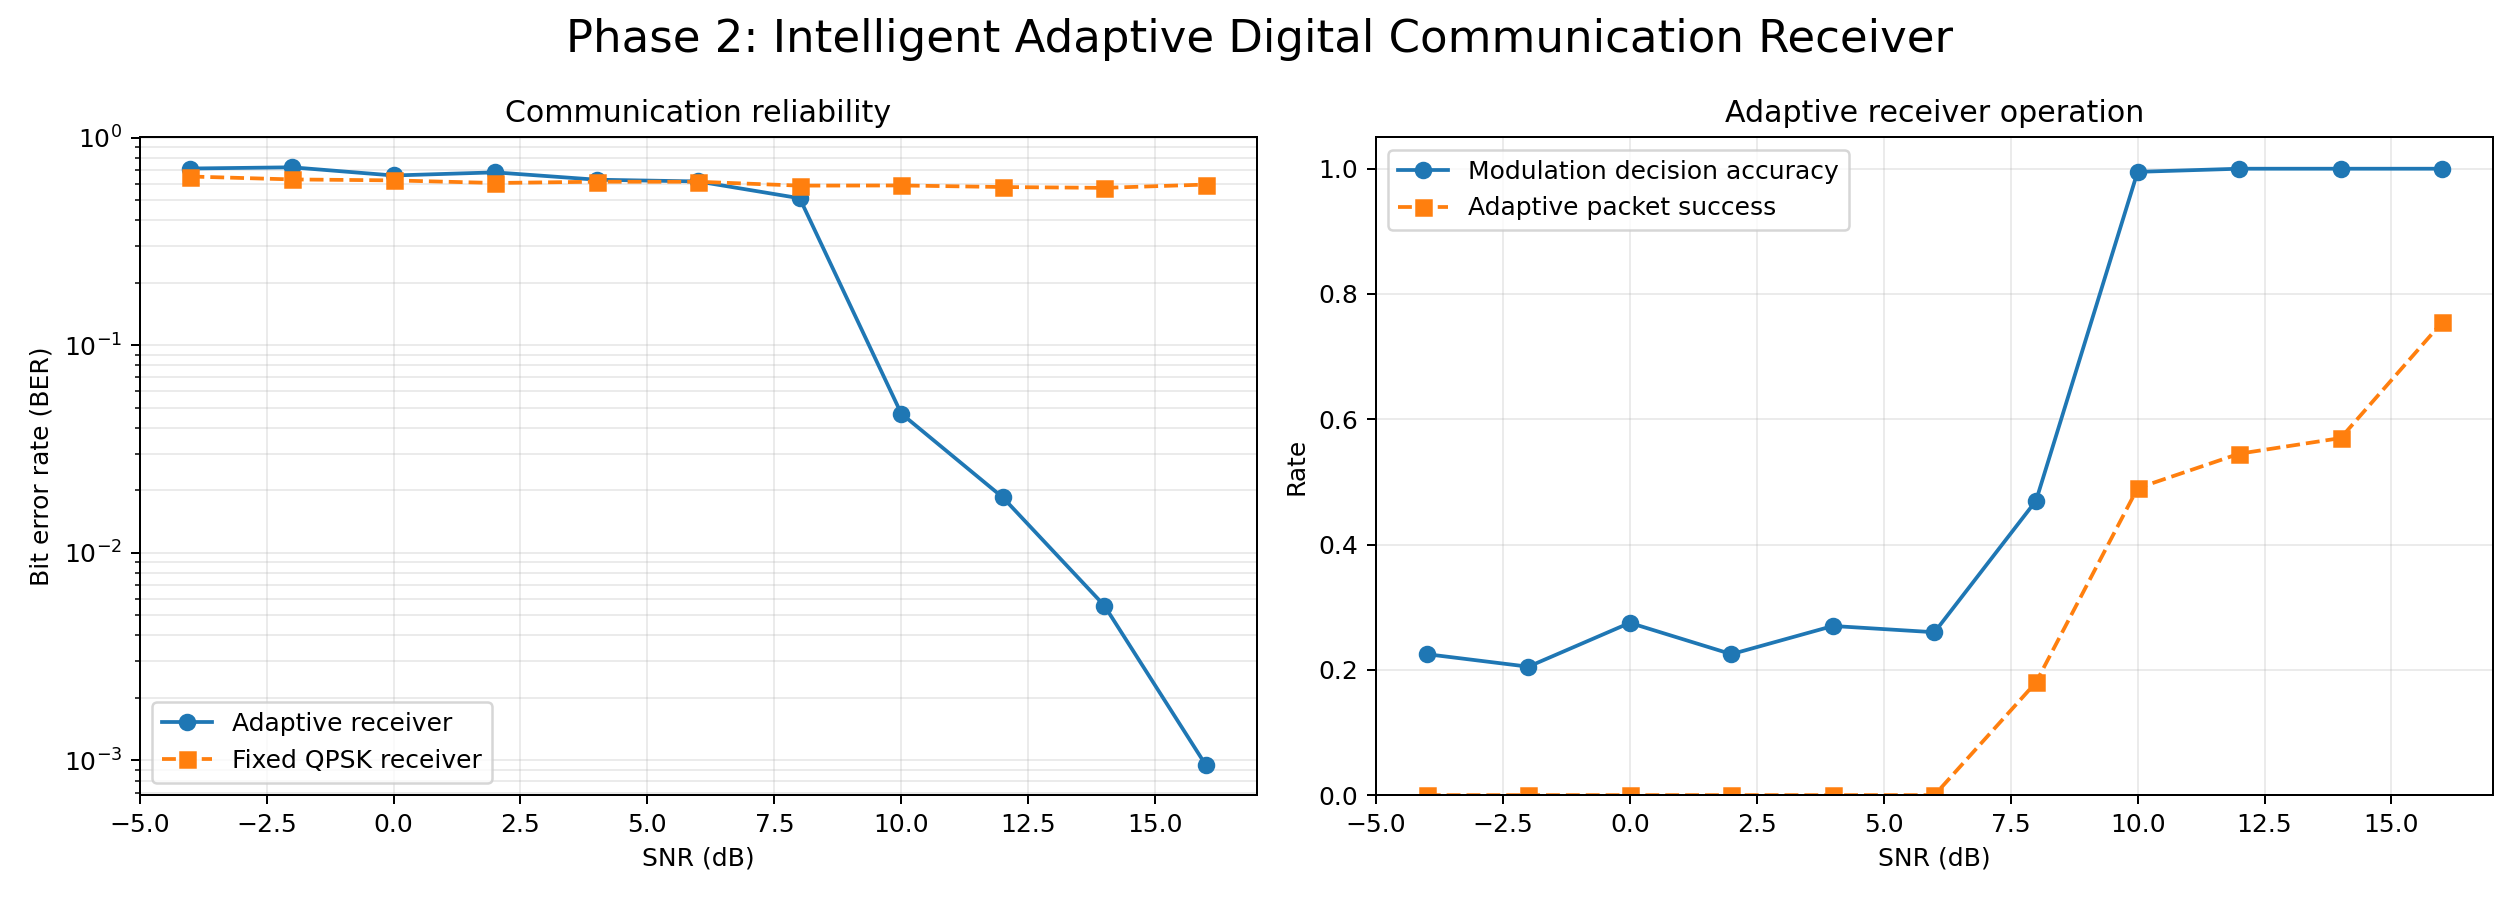
\includegraphics[width=0.91\linewidth]{artifacts/phase2-link-results.png}
\caption{Measured Phase-II BER, SER, decision accuracy, packet success, and throughput.}
\label{fig:linkresults}
\end{figure}

\section{Selected Numerical Results}
\begin{table}[H]
\centering
\small
\caption{Selected measured results from the final Phase-II experiment.}
\label{tab:selectedresults}
\begin{tabular}{c c c c c c}
\toprule
\textbf{SNR} & \textbf{BER} & \textbf{SER} & \textbf{Decision} &
\textbf{Packet} & \textbf{Throughput}\\
\midrule
10 dB & 4.69\% & 6.94\% & 99.5\% & 49.0\% & 1.225\\
12 dB & 1.85\% & 3.05\% & 100.0\% & 54.5\% & 1.363\\
14 dB & 0.56\% & 1.00\% & 100.0\% & 57.0\% & 1.425\\
16 dB & 0.095\% & 0.172\% & 100.0\% & 75.5\% & 1.888\\
\bottomrule
\end{tabular}
\end{table}

\section{High-SNR Operating Point}
At 16~dB, every modulation decision in the reported aggregate run is
correct. The remaining 0.095\% BER and 0.172\% SER are caused by residual
noise and the strict symbol decisions within correctly selected
constellations. Packet success is 75.5\%, which is lower than one minus BER
because a packet is declared successful only when all bits in its 256-symbol
frame are correct. The effective throughput reaches 1.888 bits/symbol because
successful frames contribute according to their modulation order.

\section{Transition Region}
At 10~dB, decision accuracy is already 99.5\%, but BER remains 4.69\% and
packet success is only 49.0\%. This difference is important: an accurate
format decision does not guarantee error-free communication. The receiver
can identify the correct constellation while noise still moves individual
symbols across decision boundaries. At 12~dB, the lower BER of 1.85\% and
higher packet success of 54.5\% show the beginning of the reliable operating
region.

\section{Low-SNR Failure Behavior}
At low SNR, the adaptive BER is approximately 0.71 at $-4$~dB and remains
above 0.50 through 8~dB. Decision accuracy is close to the four-format
random-choice level in the lowest region. This is not a hidden software
failure; it is the measured limit of constellation recognition under the
selected channel and estimator. It identifies where confidence thresholds,
fallback to a robust modulation, coding, or retransmission would be useful.

\section{Adaptive and Fixed-Receiver Comparison}
The fixed-QPSK reference maintains BER between approximately 0.57 and 0.65
over most of the sweep because it is mismatched to BPSK, 8-PSK, and 16-QAM
frames. In contrast, the adaptive receiver improves rapidly after the
decision transition and reaches 0.000948 BER at 16~dB. The comparison
demonstrates the practical value of receiver adaptation rather than merely
showing that a classifier can identify a label.

\section{Error Sources}
Three error sources dominate the measured behavior. First, noise causes
constellation overlap and increases estimator ambiguity. Second, fading
changes the received amplitude and can reduce the effective SNR of a frame.
Third, residual correction error moves points across decision boundaries even
when the modulation format is selected correctly. Packet success combines
all of these effects and is therefore a strict end-to-end measure.

\section{Engineering Significance}
The most important result is the change in evaluation perspective. The
receiver is not assessed only by whether it names a waveform. It is assessed
by whether the decision configures a useful demodulator and delivers
information. The Phase-II implementation therefore provides a more complete
engineering argument for adaptive communication than a standalone
classification figure.

\section{Limitations of the Results}
The synchronization estimate is pilot-assisted within the simulation and is
more controlled than an over-the-air receiver. The estimator is
constellation-based and is not yet the trained CNN operating online. The
experiment is uncoded, uses a flat block-fading model, and does not include
timing recovery, pulse shaping, multipath, Doppler, or hardware
nonlinearity. These limitations are explicitly retained so that the reported
numbers are not presented as SDR measurements.

\chapter{Conclusion and Future Work}

\section{Conclusion}
This report developed and evaluated a complete Phase-II adaptive digital
communication receiver. The system generates information bits, supports
BPSK, QPSK, 8-PSK, and 16-QAM, applies block-Rayleigh fading and AWGN with
carrier impairments, performs pilot-assisted correction, estimates the
modulation, selects a demodulator, and evaluates recovered information.

The final experiment demonstrates a clear SNR-dependent operating region.
At 16~dB, the receiver achieves 0.095\% BER, 0.172\% SER, 100\% decision
accuracy, 75.5\% packet success, and 1.888 bits/symbol throughput. At
10~dB, the 99.5\% decision accuracy but 4.69\% BER shows why communication
quality must be measured after the decision rather than inferred from it.

\section{Phase-II Contributions}
The completed work contributes a transmitter--channel--receiver architecture,
four modulation formats, configurable channel impairments, synchronization
and equalization, interpretable modulation estimation, adaptive
demodulation, a fixed-QPSK reference, reproducible metrics, figures, tests,
and an Overleaf-ready report package. These elements make the new phase
visibly different from a classification-only experiment.

\section{Limitations}
The current system is a controlled software simulation. It uses
pilot-assisted correction, an uncoded link, flat block fading, and a
constellation-distance estimator. It does not yet include a complete timing
loop, a learned classifier in the live receiver path, forward-error
correction, or over-the-air measurement.

\section{Future Work}
Future work should first implement timing recovery, carrier recovery, and
channel estimation using noisy pilots. The online estimator can then be
replaced or supplemented with a trained CNN and a confidence score. A
confidence-aware policy could select a robust fallback modulation or request
retransmission when the decision margin is small. Coding, interleaving,
frequency-selective multipath, Doppler, oscillator phase noise, nonlinear
amplification, and SDR experiments should then be added in stages.

\appendix
\chapter{Phase-II Parameter and Result Record}

\section{Fixed Experiment Parameters}
\begin{longtable}{p{0.48\textwidth} p{0.36\textwidth}}
\caption{Complete fixed parameter record for the Phase-II experiment.}
\label{tab:appendixparameters}\\
\toprule
\textbf{Parameter} & \textbf{Value}\\
\midrule
\endfirsthead
\toprule
\textbf{Parameter} & \textbf{Value}\\
\midrule
\endhead
Candidate modulation formats & BPSK, QPSK, 8-PSK, 16-QAM\\
Symbols per frame & 256\\
SNR values & $-4,-2,0,2,4,6,8,10,12,14,16$ dB\\
Frames per SNR & 200\\
Random seed & 42\\
Channel model & Block Rayleigh fading and AWGN\\
Carrier model & Random phase and frequency offset\\
Receiver correction & Pilot-assisted simulation estimate\\
Estimator & Penalized nearest-constellation distance\\
Primary output & BER, SER, decision accuracy\\
Packet output & Packet success and effective throughput\\
\bottomrule
\end{longtable}

\section{Measured Operating Points}
\begin{table}[H]
\centering
\small
\caption{Measured operating points retained in the result record.}
\label{tab:appendixresults}
\begin{tabular}{c c c c c c}
\toprule
\textbf{SNR} & \textbf{BER} & \textbf{SER} & \textbf{Decision} &
\textbf{Packet} & \textbf{Throughput}\\
\midrule
10 dB & 4.69\% & 6.94\% & 99.5\% & 49.0\% & 1.225\\
12 dB & 1.85\% & 3.05\% & 100.0\% & 54.5\% & 1.363\\
14 dB & 0.56\% & 1.00\% & 100.0\% & 57.0\% & 1.425\\
16 dB & 0.095\% & 0.172\% & 100.0\% & 75.5\% & 1.888\\
\bottomrule
\end{tabular}
\end{table}

\section{Interpretation of the Record}
The result record is the authoritative numerical source for the Phase-II
figures. The plotted curves are generated from the complete SNR arrays, while
the table above lists representative operating points for readability.
Keeping the full record prevents rounding in the report from changing the
experiment's conclusions.

\chapter{Reproducibility and Package Contents}

\section{Repository Components}
The repository is organized into communication modules, experiment drivers,
tests, generated artifacts, and report files. The communication module
contains the modulation, channel, estimator, equalizer, and demodulation
logic. The experiment driver stores the full result arrays. The figure
utilities create the report graphics from those arrays. The test suite checks
the reusable mathematical components.

\section{Reproduction Record}
The experiment is reproducible when the documented environment, seed, SNR
list, frame count, modulation set, and channel parameters are retained. The
result JSON, PNG figures, and parameter manifest are included in the package
so that a panel member can inspect both the numerical and visual outputs.

\section{Report Package Contents}
The Overleaf archive contains the single-file report, the corrected SVNIT
style file, the logo, the required empty style dependency, all referenced
Phase-II figures, numerical JSON records, source modules, experiment
utilities, and tests. All files are placed without an extra enclosing folder,
so the main TeX file and style file are visible immediately after upload.

\section{Evaluation Checklist}
\begin{itemize}
\item The title page identifies the work as a Project Phase-II Report.
\item The certificate identifies a Phase-II evaluation and academic year
      2026--27.
\item Student names and roll numbers are listed in increasing roll-number
      order.
\item Chapters 1--8 describe the Phase-II receiver rather than reproducing
      the earlier classification report.
\item Chapters 6 and 7 contain no executable command blocks.
\item Appendix A contains parameters and measured values, not program code.
\item Appendix B describes reproducibility and package contents.
\item Every figure referenced by the report is included in the archive.
\end{itemize}

\StartRef
\clearemptydoublepage
\begin{thebibliography}{99}

\bibitem{proakis2008digital}
J. G. Proakis and M. Salehi, \textit{Digital Communications}, 5th ed.,
McGraw-Hill, 2008.

\bibitem{goldsmith2005wireless}
A. Goldsmith, \textit{Wireless Communications}, Cambridge University Press,
2005.

\bibitem{azzouznandi1996}
E. E. Azzouz and A. K. Nandi,
\textit{Automatic Modulation Recognition of Communication Signals},
Springer, 1996.

\bibitem{oshea2016convolutional}
T. J. O'Shea and J. Corgan, ``Convolutional radio modulation recognition
networks,'' in \textit{IEEE Signal Processing and Machine Learning for
Communications Workshop}, 2016.

\bibitem{oshea2016generative}
T. J. O'Shea, K. Karhan, and T. C. Clancy, ``Over-the-air deep learning
based radio signal classification,'' in \textit{IEEE International
Conference on Sensing, Communication and Networking}, 2016.

\end{thebibliography}

\end{document}
